\section{Details for reproduction}
\label{app:details}

\paragraph{Items.} Facts come from the country--capital task of \citet{todd2024function} and the landmark--country, company--headquarters, star--constellation and superhero--person relations of \citet{hernandez2024linearity}; translations come from the word lists of \citet{wendler2024llamas}; arithmetic items are generated with a fixed seed (sums and differences of two-digit numbers, products of a two-digit and a one-digit number). The development and test split is made by hashing the item's subject, number pair or English word, so items that share a subject fall on the same side.

\paragraph{Known items.} The plain prompt is the item after ``Question:'', a blank line and the closing instruction, inside the model's chat template, with ``Answer:'' placed at the start of the model's reply. The gold token sequence is the shortest start of the greedy reply that matches an accepted answer after normalisation (case, accents, articles and punctuation). An item is known if this sequence exists, has at most eight tokens, and the model, given the plain prompt, assigns it a probability of at least 0.5. Table~\ref{tab:models} gives the counts.

\paragraph{Wrappers.} A seeded generator writes each wrapper from templates and a small vocabulary of office events, names and timestamps; no language model writes any wrapper text. Every wrapper is checked to contain no accepted answer of the item it wraps. Each format has 16 wrapper texts; an item uses the same text, cut to length, at all three lengths, so that everything from the question to the end is identical across lengths. The prompts in a group share all tokens before the question, which lets us compute that part once.

\paragraph{Layout.} We first ran Qwen3-4B with about 64 tokens of wrapper after the question. The fixed rule for choosing the layout was that wrappers at the longest length must lose at least 15 points more than the noise floor on development items. This layout lost \GateShortDrop{} points more, so, as planned in advance, we reran Qwen3-4B with about 512 tokens after the question, which lost \GateLongDrop{} points more. That layout is used for all models and all reported numbers, except in Appendix~\ref{app:tail}.

\paragraph{Generation.} Replies are greedy, up to 24 tokens, and stop at a newline or the end-of-turn token. Models run in bfloat16 with the Hugging Face Transformers library on one NVIDIA A100 GPU (80 GB). The whole study took \GPUHours{} GPU hours.

\begin{table}[h]
\centering
\footnotesize
\setlength{\tabcolsep}{3pt}
\begin{tabular}{@{}lcccc@{}}
\toprule
Model & Layers & Known & Known test & Pairs \\
\midrule
Qwen3-4B & 36 & 1{,}184 (74\%) & 822 & 172 \\
OLMo-3-7B & 32 & 1{,}147 (71\%) & 813 & 102 \\
Qwen3-8B & 36 & 1{,}280 (80\%) & 890 & 97 \\
Gemma-4-12B & 48 & 1{,}278 (80\%) & 895 & 106 \\
\bottomrule
\end{tabular}

\caption{\textbf{Models.} Known: items the model answers correctly in the plain prompt with probability at least 0.5, out of \NItems{}. Pairs: failed test prompts patched (Section~\ref{sec:where}).}
\label{tab:models}
\end{table}

\section{Exact-format accuracy}
\label{app:exact}
A reply is exactly right if its first line, after normalisation, is an accepted answer or starts with one followed by a space. This is what a program reading the reply would need. Table~\ref{tab:exact} compares it with the share of answers kept.

\begin{table}[h]
\centering
\footnotesize
\setlength{\tabcolsep}{3.5pt}
\begin{tabular}{@{}lcc@{}}
\toprule
Wrapper & Kept & Exactly right \\
\midrule
Tool result & 90\% & 67\% \\
Web page & 91\% & 78\% \\
Server log & 77\% & 49\% \\
Email thread & 90\% & 81\% \\
Plain prose & 88\% & 86\% \\
Neutral sentence & 99\% & 99\% \\
\bottomrule
\end{tabular}

\caption{\textbf{Kept answers and exactly right replies}, for all four models and three lengths together, test items.}
\label{tab:exact}
\end{table}

\section{Less wrapper after the question}
\label{app:tail}
Table~\ref{tab:tail} compares, for Qwen3-4B, the share of known answers kept with about 64 and about 512 tokens of wrapper between the question and the closing instruction.

\begin{table}[h]
\centering
\footnotesize
\setlength{\tabcolsep}{3.5pt}
\begin{tabular}{@{}lcc@{}}
\toprule
Wrapper & 64 tokens after & 512 tokens after \\
\midrule
Tool result & 92\% & 93\% \\
Web page & 92\% & 92\% \\
Server log & 81\% & 61\% \\
Email thread & 93\% & 93\% \\
Plain prose & 87\% & 87\% \\
\bottomrule
\end{tabular}

\caption{\textbf{Qwen3-4B: kept answers by the amount of wrapper after the question}, all three lengths together, test items.}
\label{tab:tail}
\end{table}

\section{Sorting lost answers}
\label{app:types}
We read the first line of each reply that lost the answer. It is a \emph{claim that the answer is not there} if it matches phrases such as ``provided text'', ``does not contain'', ``not mentioned'', ``not a real'' or ``does not exist''. Otherwise it is a \emph{reply about the wrapper} if it names the wrapper's content, such as logs, jobs, errors, timeouts, the email or the thread. Otherwise it is a \emph{wrong answer}. We wrote these rules after reading replies of Qwen3-4B and applied them unchanged to all models. A reply such as ``Sanaa'' for ``Sana'a'' counts as lost, so a few lost answers are spelling variants.

\begin{figure*}[t]
\centering
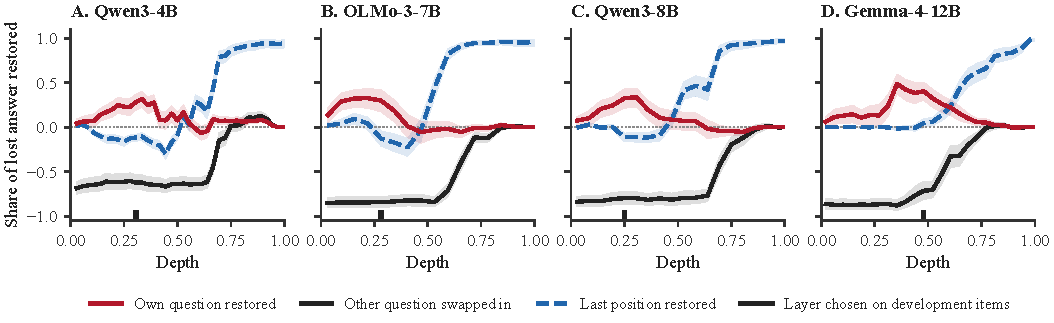
\includegraphics[width=\textwidth]{fig_repair.pdf}
\caption{\textbf{Share of the lost answer's log-probability restored} (Equation~\ref{eq:repair}), by the depth of the patch, test pairs. The tick below each axis marks $\ell^*$. Bands are 95\% intervals.}
\label{fig:repair}
\end{figure*}

\section{Patching}
\label{app:patching}

\paragraph{Which failures.} A failed prompt is eligible if its reply lost the answer, is not empty, does not begin with markup or a refusal phrase, and, for arithmetic, contains a digit; and if the model's probability of the full answer is at least three times lower than in the plain prompt. From the eligible failures we took up to \NPatchQfour{} for Qwen3-4B and \NPatchOther{} for each other model, development and test items together, cycling over item family and wrapper so that each combination is represented, with at most two prompts per item. Qwen3-4B was patched at every layer and the other models at every other layer and the last, to fit the time budget.

\paragraph{The other question.} The swapped-in question is a different known item of the same family and wording form, with the same number of question tokens, a different subject and a different first answer token. A pair is dropped if the unpatched rerun does not reproduce the failure's log-probability within 0.05 nats, which happens through small bfloat16 differences between batch shapes; this dropped \NSkipped{} pairs in the four models.

\paragraph{Positions.} A patch writes each state to the token that matches its source, counted from the start of the question; the last position is matched to the last position. The plain and wrapped prompts differ in absolute position. The models encode position by rotating the attention queries and keys, not in the residual stream, so a copied state carries no absolute position of its own.

\section{Repair of the answer's probability}
\label{app:repair}
For a failed prompt, let $\ell_{\text{plain}}$, $\ell_{\text{wrap}}$ and $\ell_{\text{patch}}$ be the log-probability of the full known answer in the plain prompt, in the wrapped prompt and in the wrapped prompt after a patch. The share of the lost answer restored is
\begin{equation}
R = \frac{\ell_{\text{patch}} - \ell_{\text{wrap}}}{\ell_{\text{plain}} - \ell_{\text{wrap}}},
\label{eq:repair}
\end{equation}
where $R = 0$ means the patch changed nothing, $R = 1$ means it restored the plain prompt's probability, and a negative $R$ means it pushed the answer further away. We clip $R$ to $[-1, 2]$. Figure~\ref{fig:repair} shows $R$ by depth. It matches Figure~\ref{fig:swap}. Swapping in another question pushes the answer away ($R$ from \DStarNeg{}) until the hand-off depth, restoring the own question recovers a part of the loss, and restoring the last position recovers it from the hand-off depth on. In the middle of the network, restoring the last position alone slightly lowers the answer's probability, before the question's content has arrived there.

We chose one layer $\ell^*$ on development pairs, where restoring minus swapping is largest, and tested it on test pairs (Table~\ref{tab:repair}). Restoring the question's states at every layer at once does not recover more than at the best single layer.



\begin{table}[h]
\centering
\scriptsize
\setlength{\tabcolsep}{2.5pt}
\begin{tabular}{@{}lcccc@{}}
\toprule
Model & $\ell^*$ & Own & Other & All layers \\
\midrule
Qwen3-4B & 10 & 0.28 [0.19, 0.37] & -0.62 [-0.70, -0.53] & 0.23 [0.11, 0.34] \\
OLMo-3-7B & 8 & 0.30 [0.17, 0.42] & -0.84 [-0.90, -0.78] & 0.12 [-0.03, 0.27] \\
Qwen3-8B & 8 & 0.33 [0.21, 0.43] & -0.80 [-0.87, -0.72] & 0.38 [0.26, 0.49] \\
Gemma-4-12B & 22 & 0.41 [0.30, 0.51] & -0.71 [-0.81, -0.60] & 0.34 [0.20, 0.47] \\
\bottomrule
\end{tabular}

\caption{\textbf{Repair at $\ell^*$}, test pairs, with 95\% intervals. Own: own question restored. Other: other question swapped in. All layers: own question restored at every layer at once.}
\label{tab:repair}
\end{table}
